\section{Konzept}

    \subsection{Architektur}
    \begin{figure}[H]
        \centering
        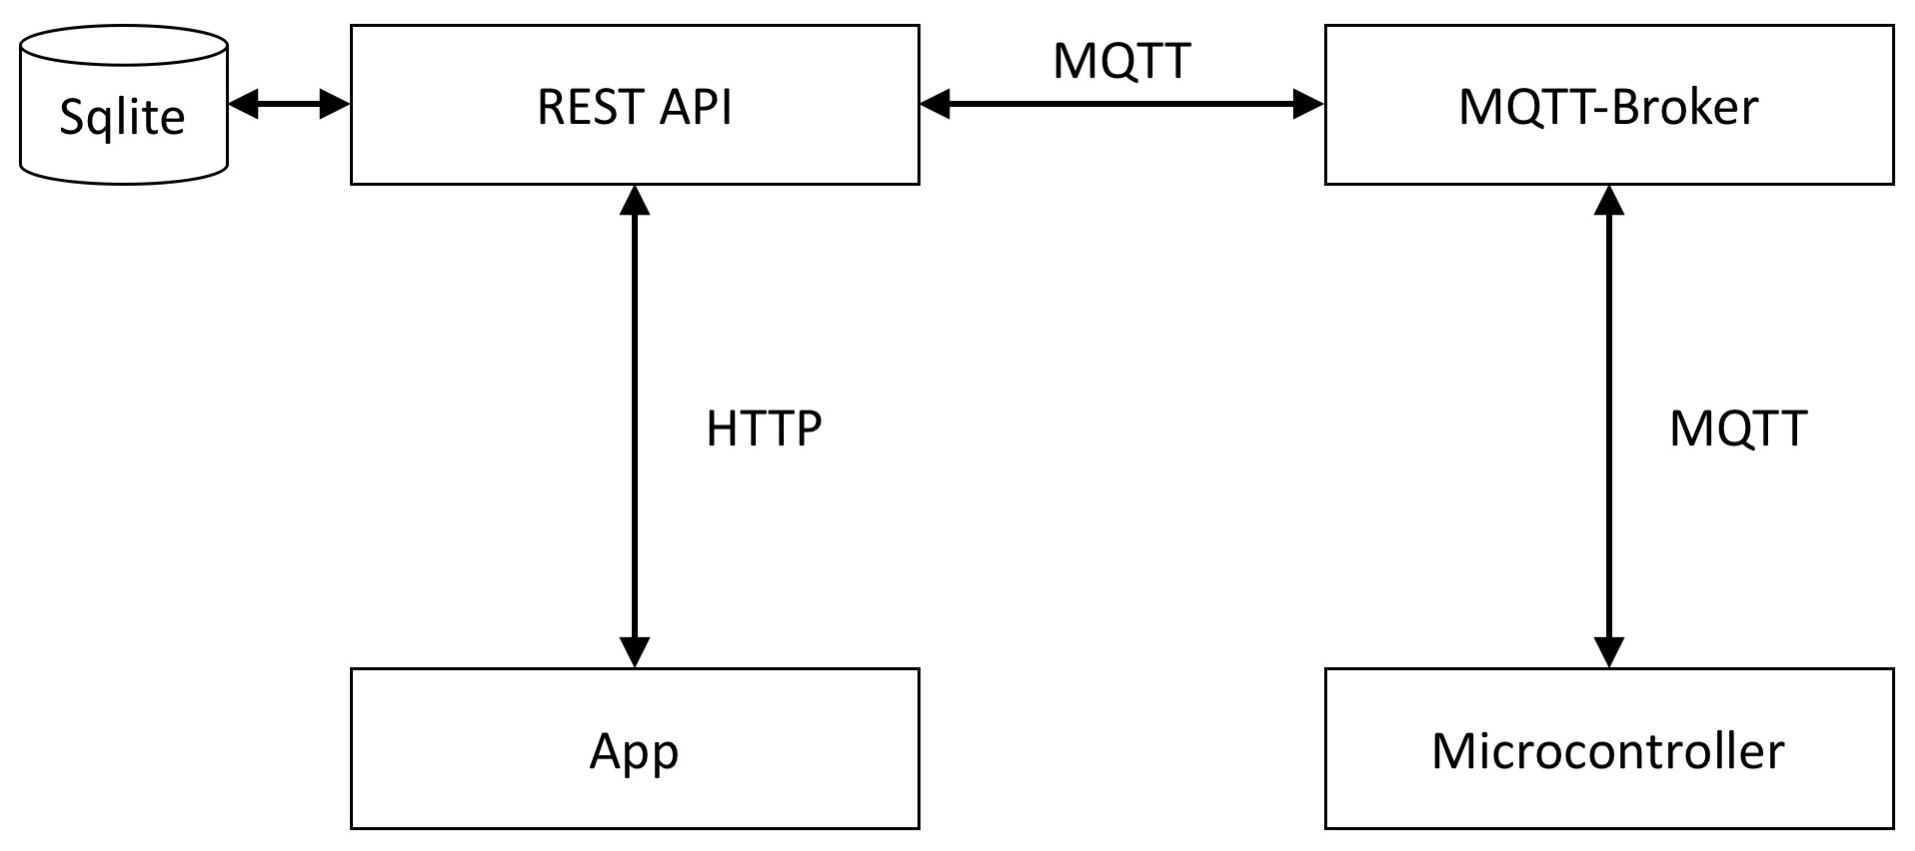
\includegraphics[width=0.7\linewidth]{../Pictures/Konzept/Architecture}
        \caption{Projektarchitektur}
        \label{fig:architecture}
    \end{figure}
    
    \subsection{Datenmodell}
    
    \subsection{Mobile Applikation}

        \subsubsection{React Native}
        \subsubsection{Views}

    \subsection{REST-API}

        \subsubsection{Django}
        \subsubsection{Ressourcen}
        \newcommand{\tabitem}{~~\llap{\textbullet}~~}
        
         GET controller/\{controllerID\}/ 
        
          \begin{tabularx}{\textwidth}{lX}
                Beschreibung & Überprüft Validität der Controller-ID \\
                URL-Parameter & controllerID: zu überprüfende ID des Controllers \\
                Body & - \\
                Response & \{ "exists": true/false\}
            \end{tabularx}\\
        
        GET controller/\{controllerID\}/plant/ 

          \begin{tabularx}{\textwidth}{lX}
                Beschreibung & Alle Pflanzen des Microcontrollers \\
                URL-Parameter & controllerID: ID des Controllers mit dem die Pflanzen verbunden sind \\
                Body & - \\
                Response & Liste von Pflanzen
            \end{tabularx}\\
        
         POST  controller/\{controllerID\}/plant/ 
         
          \begin{tabularx}{\textwidth}{lX}
             Beschreibung & Erstellt eine neue Pflanze \\
             URL-Parameter & controllerID: ID des Controllers mit dem die Pflanzen verbunden sind \\
             Body & Zu erstellende Pflanze ohne ID \\
             Response & Erstellte Pflanze mit ID
         \end{tabularx}\\
     
          GET  controller/\{controllerID\}/plant/\{plantID\} 
          
          \begin{tabularx}{\textwidth}{lX}
              \toprule Beschreibung & Alle Informationen zu einer spezifischen Pflanze \\
              URL-Parameter & 
                  \begin{tabular}[t]{ll}
                       \tabitem controllerID: ID des Controllers mit dem die Pflanzen verbunden sind \\ 
                       \tabitem plantID: Eindeutige ID der angefragten Pflanze
                  \end{tabular}\\
              Body & - \\
              Response & Pflanzenobjekt
          \end{tabularx}\\
          
          PUT controller/\{controllerID\textgreater/plant/\{plantID\} 
          
            \begin{tabularx}{\textwidth}{lX}
              \toprule Beschreibung & Updated eine existierende Pflanze \\
              URL-Parameter & 
              \begin{tabular}[t]{ll}
                  \tabitem controllerID: ID des Controllers mit dem die Pflanzen verbunden sind \\ 
                  \tabitem plantID: Eindeutige ID der zu updatenden Pflanze
              \end{tabular}\\
              Body & Geändertes Pflanzenobjekt \\
              Response & Geändertes Pflanzenobjekt
          \end{tabularx}\\
      
          DELETE controller/\{controllerID\}/plant/\{plantID\}/ 
          
          \begin{tabularx}{\textwidth}{lX}
              \toprule Beschreibung & Löschen einer Pflanze \\
              URL-Parameter & 
              \begin{tabular}[t]{ll}
                  \tabitem controllerID: ID des Controllers mit dem die Pflanzen verbunden sind \\ 
                  \tabitem plantID: Eindeutige ID der zu löschenden Pflanze
              \end{tabular}\\
              Body & - \\
              Response & -
          \end{tabularx}\\
      
          GET  controller/\{controllerID\}/plant/\{plantID\}/moisture 
          
          \begin{tabularx}{\textwidth}{lX}
              \toprule Beschreibung & Abfragen aller Feuchtigkeitsmessungen für eine Pflanze \\
              URL-Parameter & 
              \begin{tabular}[t]{ll}
                  \tabitem controllerID: ID des Controllers mit dem die Pflanzen verbunden sind \\ 
                  \tabitem plantID: Eindeutige ID der Pflanze
              \end{tabular}\\
              Body & - \\
              Response & Liste an Feuchtigkeitswerten
          \end{tabularx}\\
      
      POST controller/\{controllerID\}/plant/\{plantID\}/water/\{amount\} 
      
      \begin{tabularx}{\textwidth}{lX}
          \toprule Beschreibung & Bewässerung einer Pflanze \\
          URL-Parameter & 
          \begin{tabular}[t]{ll}
              \tabitem controllerID: ID des Controllers mit dem die Pflanzen verbunden sind \\ 
              \tabitem plantID: Eindeutige ID der zu bewässernden Pflanze \\
              \tabitem amount: Wassermenge in Millilitern
          \end{tabular}\\
          Body & - \\
          Response & -
      \end{tabularx}\\
  
%        \begin{table}[]
%            \centering
%            \caption{My caption}
%            \label{my-label}
%            \begin{tabular}{|l|l|l|}
%                \hline
%                Typ    & URL                                                            & Beschreibung                                       \\ \hline
%                GET    & controller/\{controllerID\}/                                   & Validierung der ID des Microcontrollers            \\ \hline
%                GET    & controller/\{controllerID\}/plant/                             & Alle Pflanzen des Microcontrollers                 \\ \hline
%                POST   & controller/\{controllerID\}/plant/                             & Erstellung einer neuen Pflanze                     \\ \hline
%                GET    & controller/\{controllerID\}/plant/\{plantID\}                  & Alle Informationen zu spezifischer Pflanze         \\ \hline
%                PUT    & controller/\{controllerID\textgreater/plant/\{plantID\}        & Updaten einer existierenden Pflanze                \\ \hline
%                DELETE & controller/\{controllerID\}/plant/\{plantID\}/                 & Löschen einer Pflanze                              \\ \hline
%                GET    & controller/\{controllerID\}/plant/\{plantID\}/moisture         & Alle Feuchtigkeitswerte einer Pflanze              \\ \hline
%                POST   & controller/\{controllerID\}/plant/\{plantID\}/water/\{amount\} & Bewässerung einer Pflanze mit Menge in Millilitern \\ \hline
%            \end{tabular}
%        \end{table}

    \subsection{Microcontroller}

        \subsubsection{Kommunikation}
        \subsubsection{Verwendete Hardwarekomponenten}

    \subsection{Codequalität}